\documentclass[sigconf]{acmart}
% The preceding line is only needed to identify funding in the first footnote. If that is unneeded, please comment it out.
% On windows run updmap
\usepackage{amsmath,amsfonts}
\usepackage{algorithmic}
\usepackage{graphicx}
\usepackage{textcomp}
\usepackage{listings}
\usepackage{xcolor}
\usepackage{multirow}
\usepackage{dcolumn}
\usepackage{booktabs} 
\usepackage{pifont}  % use /ding{55} for X... /ding{51} for check
\usepackage{url}
\usepackage{hyperref}
\usepackage{adjustbox}
\usepackage{threeparttable}
\usepackage[nameinlink]{cleveref}

\expandafter\newcommand\csname r@tocindent4\endcsname{4in}
\setcounter{secnumdepth}{4}
\setcounter{tocdepth}{4}

\lstset{
language=Java,
basicstyle=\small\ttfamily,			
keywordstyle=\color{blue},
commentstyle=\color{gray},			
stringstyle=\color{black},					
}


\AtBeginDocument{%
  \providecommand\BibTeX{{%
    \normalfont B\kern-0.5em{\scshape i\kern-0.25em b}\kern-0.8em\TeX}}}

% My 'newcommand' for modulo function...
\newcommand{\abs}[1]{\left|#1\right|}


% My 'newcommand' for standard table creation...
\newcommand{\AndreaTable}[3]{\begin{table*}[h!]
\caption{#1}
\centering
\begin{tabular}{#2}
\toprule
#3
\bottomrule
\end{tabular}
\end{table*}
}

% My 'newcommand' for standard table creation...
\newcommand{\equivalenceClassesTable}[2]{
\AndreaTable{#1}{llm{8cm}m{8cm}}{#2}
}


\definecolor{beaublue}{rgb}{0.74, 0.83, 0.9}


\settopmatter{printacmref=false, printccs=false, printfolios =false}
\setcopyright{none} 
\renewcommand\footnotetextcopyrightpermission[1]{}
\acmConference[ISW2 Project A.A. 2019-2020]{ }{September 1, 2020}{ }

\begin{document}

\title{ISW2 Project A.A. 2019-2020}

\author{Andrea Graziani ($0273395$)}
\email{andrea.graziani93@outlook.it}
\affiliation{
  \institution{Università degli Studi di Roma "Tor Vergata"}
  \city{Rome}
  \country{Italy}
}

\keywords{Testing, Equivalence Class Partitioning, Boundary Value Analysis, Mutation Testing}
\maketitle

\section{Introduction}

Why are some programs more defect-prone than others? 

This is one of the central questions of software engineering. To answer it, we must first know \textit{which} programs or software modules are more failure-prone than others, afterwards, with this knowledge, we can search for properties of the program that are correlate with defect density. How to do that?

Let's start now with some definitions. A \textbf{software defect} can be generally considered as an error, flaw, bug, mistake, failure, or fault in a computer program or system that may generate an inaccurate or unexpected outcome, or precludes the software from behaving as intended \cite{SoftwareDefectPredictionRawat}.

Software defects always incur cost in terms of time because identifying and rectifying defects is one of the most time consuming and expensive software processes \cite{SoftwareDefectPredictionRawat}.

Although it's not practically possible to eliminate each and every defect from a software product, we can reduce their adverse effects exploiting \textbf{software defects prediction} techniques, which aim is to identify software modules that are defect prone, in order to reduce the cost of testing activities and code review by letting developers focus on specific artefacts \citep{Falessi}.

How to build a software defect prediction model? 

The building of a software prediction model based on \textbf{machine learning} techniques passes through several steps which we will describe them in following sections.

\subsection{Dataset building}

Firstly, is necessary to generate a data-set to provide an appropriate input for our prediction model, that is we need to build a set of \textbf{instances}. In our context, each data-set's instance represents a \textbf{source code file} belonging to an open-source software project and characterized by its values on a fixed, predefined set of \textbf{features}, or \textbf{attributes}.

Clearly, in order to build an useful software predictor, is preferable to collect instances whose features are correlated to the defect-proneness of the software module they belong. Fortunately, there are many studies about software defect-proneness which have identified several features (sometimes called also \textbf{metrics}) correlated with defect density of a software module. 

For example, \citet{PredictingDefectsForEclipse} showed that the number of past defects has the highest correlation with number of future defects. \citet{Nagappan} report that \textit{code churn} is a very powerful metric for predict software defect density, while \citet{Gyimothy} showed the same with \textit{lines of code} (\texttt{LOC}) metric.

Defect-proneness correlated features are extracted from \textit{history data} of software module, including software archives and tools like \textit{version control systems} and \textit{issue tracking systems}, because they are generally assumed as a good source for future fault prediction. 

\subsection{Labelling activity}

Since our aim is to build a software defect predictor using a \textit{supervised learning scheme}, is necessary to perform the so-called \textit{labelling} task, that is an activity according to which one or more informative tags are assigned to each unlabelled instance of a given dataset.

In fact, when a supervised learning scheme is used, the goal is to learn a function that maps an input to an output based on example input-output pairs. In other word, each data-set instance $T$ is represented as a pair $(x_{d}, y)$ where $x_d$ is a $d$-dimensional input object while $y$ is the desired output value. In this way, a supervised learning algorithm, analysing labelled training data, can produce an inferred function, which can be used for mapping new instances.

In our context, to build a properly data-set, we need to label each instance as \textit{buggy} or \textit{not buggy}. 

In order to do that during the development of our predictor, we have exploited all information retrievable both from \texttt{JIRA}\footnote{\url{https://www.atlassian.com/it/software/jira}}, one of the most popular issue tracking systems, and \texttt{git}\footnote{\url{https://git-scm.com/}}, the most common version control systems.

\begin{lstlisting}[frame=lines,basicstyle=\ttfamily\tiny, caption={Dataset build logic}, label={buildProjectDataset}]
public void buildProjectDataset() {

        collectReleases();
        collectFilesBelongingToEachRelease();

        IssueRegistry issueRegistry = this.issueTrackingSystem.getIssuesRegistry(this.project.name, this.releasesByVersionID);

        calculateDefectiveFileProportion(issueRegistry.issuesWithAffectedVersions);
        searchForDefectiveFile(issueRegistry.issues);

        collectFileMetadataOfEachRelease();
    }
\end{lstlisting}

First of all, it is necessary to identify all project's releases.

To do that, we have simply queried \texttt{Jira} to obtain all releases data, including names, release dates and so on. Subsequently, we have exploited \texttt{git} tags inside commits messages to identify the commit associated to each release. However, when sometimes \texttt{git} tags were not available, we have identified aforementioned commits exploiting \texttt{git log} command with \texttt{--before [date]} options. \texttt{collectReleases} method, inside \texttt{ProjectDatasetBuilder}\footnote{\texttt{datasetbuilder.ProjectDatasetBuilder}} class, contains the implementation of this step.

To discover all known bugs, we have queried once again \texttt{Jira} to obtain the identifiers of all issues with type \texttt{"Bug"} and status \texttt{"Closed"} (or \texttt{"resolved"}). We remember that is possible to find the implementation of this query procedure inside \texttt{getIssuesRegistry} method into \texttt{Jira} class \footnote{\texttt{datasetbuilder.datasources.its.jira.Jira}}.

Is very important to precise that scientific literature reports that most of the projects have more than $25\%$ of defects whose issue report contained no \textit{"Affected Version"} (\textbf{AV}). Moreover, the vast majority of all bugs ($51\%$) resulted in not having or having an unreliable AV. Therefore, if information about the AV for a bug is available in \texttt{Jira}, we will consider the earliest AV in Jira to be the release that introduced the bug, otherwise we have adopted proportion method.

However, the creation of such datasets made in this way is far from being perfect because scientific literature reports that most of the projects have more than $25\%$ of defects whose issue report contained no AV. Moreover, the vast majority of all bugs (51\%) resulted in not having or having an unreliable AV.







\begin{table*}


\begin{tabular}{l|p{6cm}}

\toprule
\textbf{Name} & \textbf{Description} \\
\midrule

\\

\texttt{LOC} & Lines of code of $X$. 

\\

\texttt{LOC\_TOUCHED} & $\sum_R (\texttt{addedLOC} + \texttt{deletedLOC})$, where: 

\begin{itemize}
\item $R$ is the set of all revisions of $X$.
\item $\texttt{addedLOC}$ represents the number of added code lines while $\texttt{deletedLOC}$ represents the removed ones.
\end{itemize}

\\

\texttt{LOC\_ADDED} & $\sum_R (\texttt{addedLOC})$

\\

\texttt{MAX\_LOC\_ADDED} & $\max_R (\texttt{addedLOC})$.

\\
    
\texttt{AVERAGE\_LOC\_ADDED} & $\dfrac{\sum_R (\texttt{addedLOC})}{\mid R \mid}$

\\

\texttt{NUMBER\_OF\_REVISIONS} & $\mid R \mid$ 

\\

\texttt{NUMBER\_OF\_FIX} & Number of bug fixes which have involved $X$.

\\

\texttt{NUMBER\_OF\_AUTHORS} & Number of authors which developed $X$.

\\

\texttt{CHURN} & $\sum_R (\texttt{addedLOC} - \texttt{deletedLOC})$

\\

\texttt{MAX\_CHURN} & $\max_R (\texttt{addedLOC} - \texttt{deletedLOC})$

\\

\texttt{AVERAGE\_CHURN} & $\dfrac{\sum_R (\texttt{CHURN})}{\mid R \mid}$

\\

\texttt{MAX\_CHANGE\_SET\_SIZE} &

\\

\texttt{AVERAGE\_CHANGE\_SET\_SIZE} &

\\

\texttt{AGE\_IN\_WEEKS} & 

\\

\texttt{WEIGHTED\_AGE\_IN\_WEEKS} & 

\\

\bottomrule
\end{tabular}
\end{table*}

\subsection{Preprocessing}

After generating our data-set, according to project specifications, we have also applied a preprocessing technique, commonly used in machine learning, called \textbf{feature selection} or \textbf{attribute selection}. 

\subsubsection{Introduction}
\hfill\\
As known, most machine learning algorithms are designed to learn which are the most appropriate attributes to use for making their decisions. For example, decision tree methods choose the most promising attribute to split on at each point and should never select irrelevant or unhelpful attributes \cite{FalessiDataMining}. 

Although, theoretically, having more attributes give us a more discriminating power, in practice, adding irrelevant attributes to a dataset, often performance of machine learning systems degrades \cite{FalessiDataMining}. 

Deleting unsuitable attributes using any feature selection algorithm, is possible to \textbf{improve learning algorithms performances}, although, using specific data-sets, is possible that these techniques \textbf{can require extensive computations}, degrading overall performances. This is the reason according to which, as in many others machine learning situations, trial and error, using specific source of data, is the best choice \cite{FalessiDataMining}.

How to select relevant features?

Clearly, the best way to select relevant attributes is \textit{manually}, based on a deep understanding of the learning problem. however, fortunately, automatic methods exist too. In fact, for our analysis, according to project specifications, we have adopted \textbf{Best-first} search method. 

This scheme adopts a \textit{greedy approach} to select attribute subset that is most likely to make better predictions. Its peculiarity it that it does not just terminate when the performance starts to drop but keeps a list of all attribute subsets evaluated so far, sorted in order of the performance measure, so that it can revisit an earlier configuration instead \cite{FalessiDataMining}. 

\subsubsection{Results analysis}
\hfill\\
Comparing results derived from our dataset processed using Best First search method with those processed without feature selection algorithms, we have noted that Best First method is capable to \textbf{improve the accuracy of specific classifiers}.
 
In fact, as you can see from \textbf{\cref{fig:BOOKKEEPER:FeatureSelectionWithoutSampling}}, containing prediction evaluation of BookKeeper dataset, when a \textit{Naive Bayes} classifier is used (without any sampling scheme), exploiting Best First method, we have obtained following results:

\begin{itemize}
\item \textit{Recall} parameter increased by $27.72\%$, passing from a value equal to $0.440$ to $0.562$. 
\item \textit{Kappa} parameter increased by $40.22\%$, from $0.179$ to $0.251$. 
\item \textit{ROC} parameter increased by $2.47\%$, from $0.686$ to $0.703$.
\item \textit{Precision} parameter decrease by $1.94\%$, from $0.630$ to $0.618$.
\end{itemize}
 
In summary, our experiments show that Naive Bayes classifier improves its accuracy when Best First is used. 

However, using others classifiers, we have obtained very different results. For example, when \textbf{Random Forest} classifier is used, our experiment results show that: 

\begin{itemize}
\item \textit{Recall} parameter decreased by $12,5\%$, passing from a value equal to $0.612$ to $0.544$. 
\item \textit{Kappa} parameter decreased by $25.28\%$, from $0.446$ to $0.356$. 
\item Both \textit{ROC} and \textit{Precision} parameters decreased by $2.87\%$ and $4.84\%$ respectively.
\end{itemize}

\textbf{IBK} classifier shows results very similar to those of Random Forest too.

\begin{figure*}[h]
  \centering
  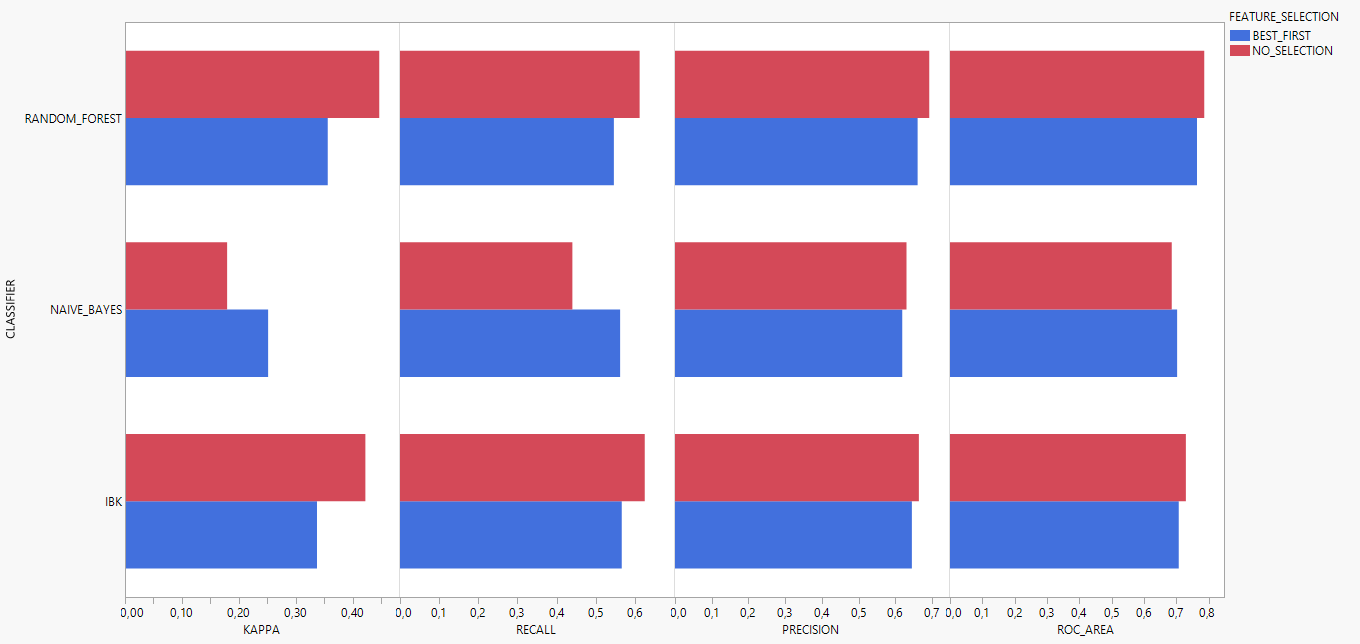
\includegraphics[width=\linewidth]{1 - BOOKKEEPER - FeatureSelectionWithoutSampling.png}
  \caption{System Architecture}
  \label{fig:BOOKKEEPER:FeatureSelectionWithoutSampling}
\end{figure*}

\subsubsection{Sampling}
\hfill\\

As known, performance of a software defect prediction model depends heavily on the data on which it was trained. In fact, defect prediction models that are trained on imbalanced datasets, that is datasets where the proportion of defective and clean modules is not equally represented, are highly susceptible to producing inaccurate prediction models \cite{FalessiSampling}

To mitigate the risk of imbalanced datasets during our analysis, we have adopt following class rebalancing techniques.

\begin{description}
\item[Over-sampling] It randomly samples with replacement the minority class to be the same size as the majority class. It is also known as up-sampling.

\item[Under-sampling] It samples the majority class in order to reduce the number of majority modules to be the same number as the minority class. It is also known as down-sampling.

\item[SMOTE] This technique combats the disadvantages of both over-sampling and under-sampling techniques, creating artificial data based on the feature space similarities from the minority class. 

\end{description}

\subsubsection{Results analysis}
\hfill\\
Comparing results derived from our dataset processed using Best First search method with those processed without feature selection algorithms, we have noted that Best First method is capable to \textbf{improve the accuracy of specific classifiers}.

As you can see from \textbf{\cref{fig:BOOKKEEPER:SamplingNoFeatureSelection}}, concerning
Concernging 

\begin{itemize}
\item Independently from used classifier, concerning \textit{Recall} parameter, under-sampling technique perform better than all other sampling techniques.

\item When Naive Bayes classifier is used, our results state that, in order to achieve better predictions accuracy, SMOTE technique performs better than any other. 

In fact, we were able to reach maximum value of Kappa and ROC parameter, while precision is very slightly less than result obtained with no sampling. 

\end{itemize}






 


\begin{figure*}[h]
  \centering
  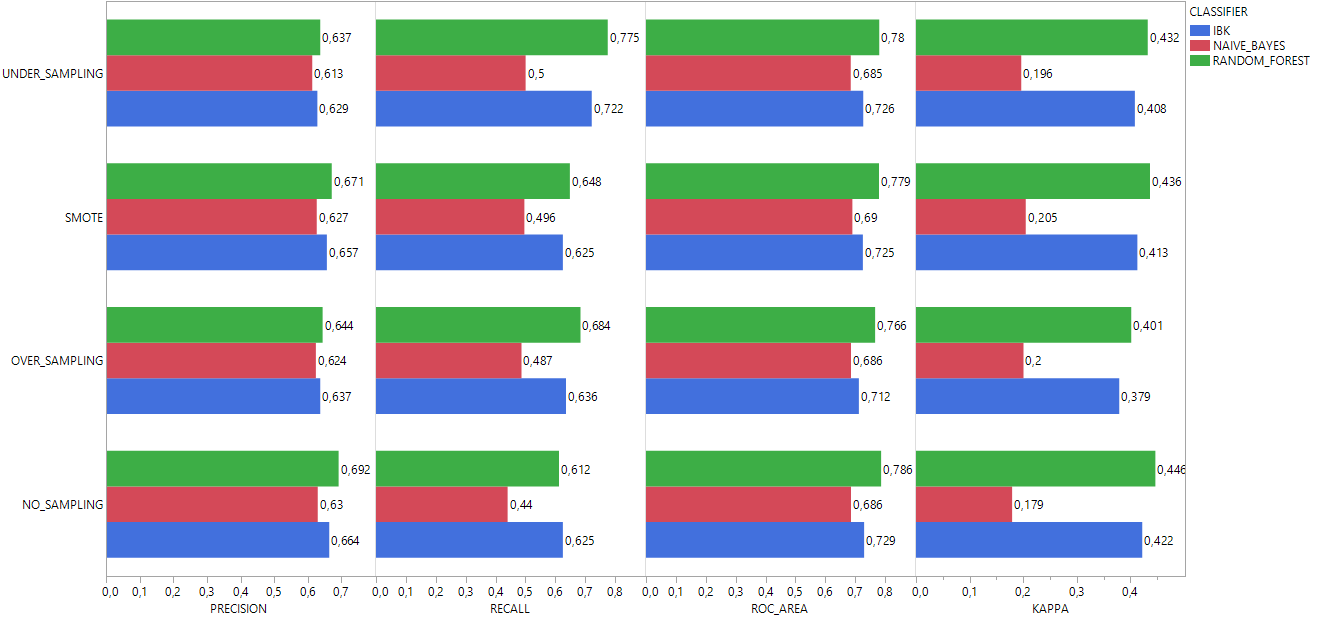
\includegraphics[width=\linewidth]{1 - BOOKKEEPER - SamplingNoFeatureSelection}
  \caption{System Architecture}
  \label{fig:BOOKKEEPER:SamplingNoFeatureSelection}
\end{figure*}







\bibliographystyle{ACM-Reference-Format}
\bibliography{bib}


\end{document}
\endinput


